\section{Introduction}

\begin{frame}{Motivation: multiphase flow simulation software}

    \begin{center}
    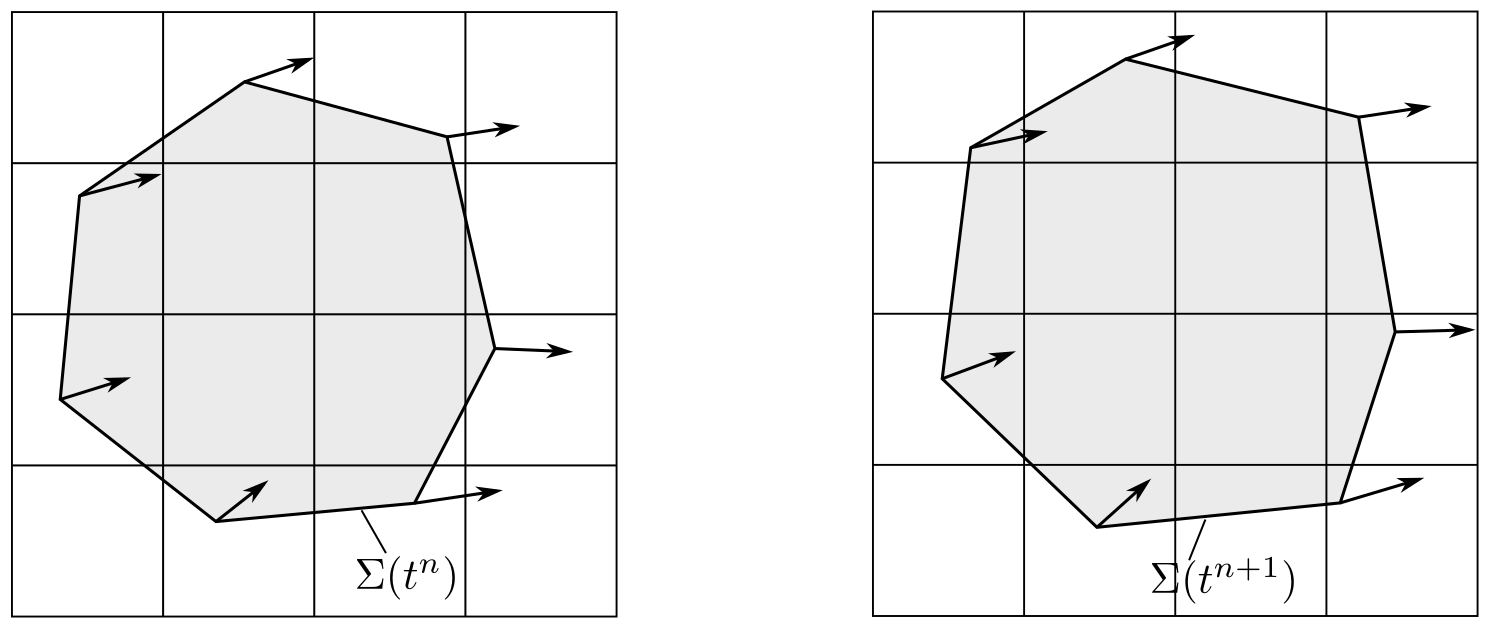
\includegraphics[width=0.7\textwidth]{figures/interface.png}
    \end{center}
    \begin{itemize}
        \item Fluids that do not mix are separated by an interface $\Sigma(t)$ (surface in 3D). 
        \item Goal: track $\Sigma(t)$ as it moves in time $t$ and changes its topology. 
    \end{itemize}

\end{frame}

\begin{frame}{Motivation: multiphase flow simulation software}
    \framesubtitle{Lagrangian / Eulerian Interface Advection (LEIA) Methods}

    \vfill
    LEIA methods\footnote{Marić, T., Marschall, H., \& Bothe, D. (2015). lentFoam–A hybrid Level Set/Front Tracking method on unstructured meshes. Computers \& Fluids, 113, 20-31.}\textsuperscript{,}\footnote{\footnotesize Tolle, T., Bothe, D., \& Marić, T. (2020). SAAMPLE: A Segregated Accuracy-driven Algorithm for Multiphase Pressure-Linked Equations. Computers \& Fluids, 200, 104450.}\textsuperscript{,}\footnote{Marić, T., Kothe, D. B., \& Bothe, D. (2020). Unstructured un-split geometrical Volume-of-Fluid methods–A review. Journal of Computational Physics, 420, 109695.} require thorough testing: 
    \begin{itemize}
        \item Verification cases: evolution of $\Sigma(t)$ and two-phase flows with exact solutions. 

        \item Validation with respect to experiments.  

        \item Serial and parallel computational efficiency. 
    \end{itemize}

\end{frame}

%\begin{frame}{Motivation: Level Set / Front Tracking method\footnote{\footnotesize Marić, T., Marschall, H., \& Bothe, D. (2015). lentFoam–A hybrid Level Set/Front Tracking method on unstructured meshes. Computers \& Fluids, 113, 20-31.},\footnote{\footnotesize Tolle, T., Bothe, D., \& Marić, T. (2020). SAAMPLE: A Segregated Accuracy-driven Algorithm for Multiphase Pressure-Linked Equations. Computers \& Fluids, 200, 104450.}}

    %\vfill
    %\begin{center}
        %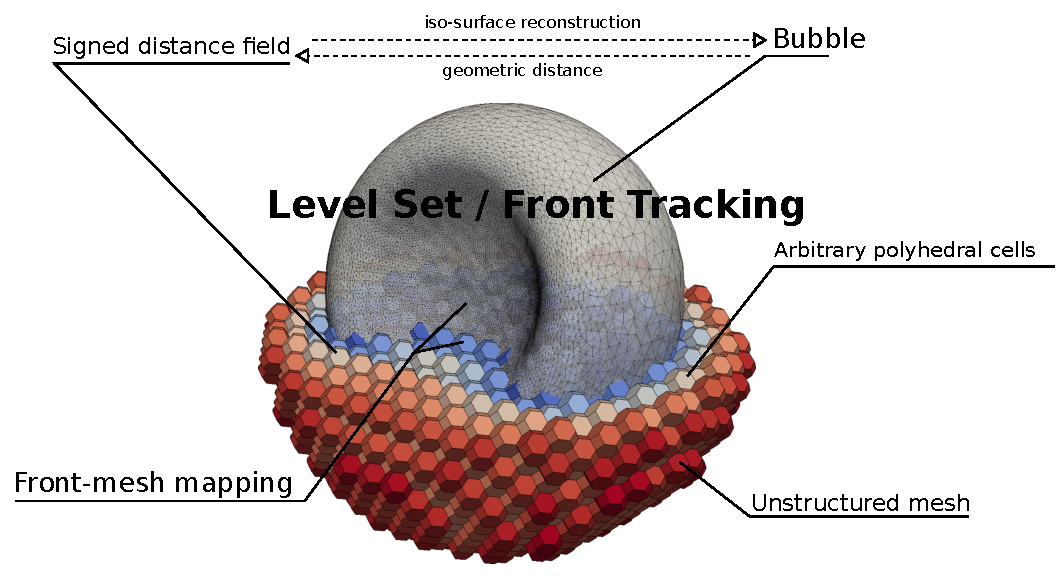
\includegraphics[width=0.5\textwidth]{figures/lent-schematic.pdf}
    %\end{center}
%\end{frame}

%\begin{frame}{Motivation: geometrical un-split Volume-of-Fluid method\footnote{Marić, T., Kothe, D. B., \& Bothe, D. (2020). Unstructured un-split geometrical Volume-of-Fluid methods–A review. Journal of Computational Physics, 420, 109695.}}

    %\vfill
    %\begin{center}
        %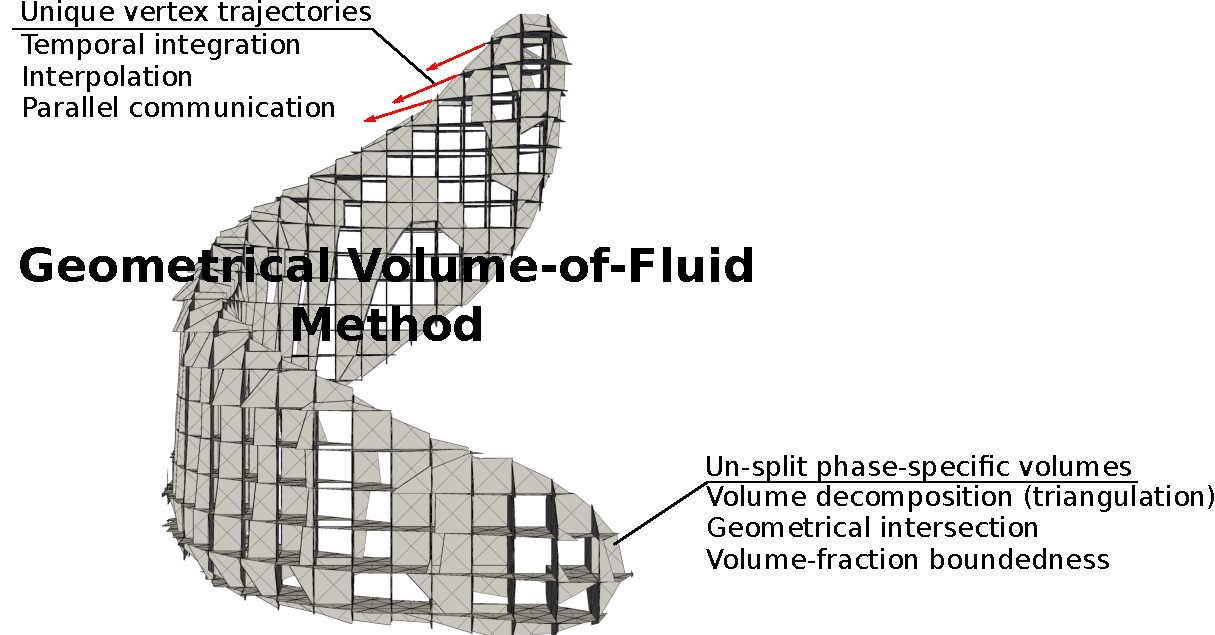
\includegraphics[width=0.6\textwidth]{figures/geovof-schematic.pdf}
    %\end{center}

%\end{frame}

\begin{frame}{Computational Science and Engineering software in\\university research groups}
	\framesubtitle{Boundary and initial conditions}
	
	\vfill
	\begin{itemize}
            \item Publish or perish \faGraduationCap\footnote{Symbol of a publish-or-perish simplification of the workflow :)} prioritizes publications over scientific software.
		\item Dedicated resources for increasing software quality are usually not available.
		\item Ph.D. students rotate every ~4-5 years, postdocs every 1-2 years. 
			\begin{itemize}
				\item Little or no overlap between successors and predecessors. 
			\end{itemize}
		\item Large-scale software design is not a necessary part of the CSE curriculum. 
			\begin{itemize}
				\item Different CSE background: (Applied) Mathematics, Mechanical Engineering, Physics, Informatics.
			\end{itemize}
		\item Real-world example: onboarding people into \href{https://www.openfoam.com/documentation/guides/latest/api/classes.html}{\beamergotobutton{OpenFOAM}} module development.
	\end{itemize}
\end{frame}

\begin{frame}{Computational Science and Engineering software in\\university research groups}
	\framesubtitle{Divergence}
	
	\vfill
	\begin{itemize}
            \item Not being able to continue development from an earlier state.
            \item Reproducing results from a publication is not possible.  
                \begin{itemize}
                    \item Data, source code and publication are not archived and cross-linked. 
                    \item The version used to generate the data is not documented. 
                \end{itemize}
            \item Not being able to re-use a model from a publication. 
                \begin{itemize}
                    \item The model is not implemented in a modular way.
                    \item Version integration was not done.
                    \item Non-granular commits were used. 
                \end{itemize}
            \item Having no overview of the impact of a change on the rest of the module.
	\end{itemize}

	\medskip

\end{frame}

\begin{frame}{Similarity with other workflows / best practices}

	\vfill
	Our \emph{(subjective)} estimates* of similarity $1-5$ (higher is more similar), $-$: aspect not addressed.
	\begin{center}
		\scriptsize
		\begin{tabular}{@{} *6l @{}}    \toprule
				\emph{DOI} & \emph{Branching model} & \emph{TDD} & \emph{Cross-linking} & \emph{CI}  & (Meta)data standardization \\\midrule
				 \href{https://doi.org/10.12688/f1000research.11407.1}{10.12688/f1000research.11407.1} 
					 & -  & -  & -  & - & 1  \\ 
				 \href{https://doi.org/10.3934/math.2016.3.261}{10.3934/math.2016.3.261} 
					 & -  & -  & -  & - & 2  \\ 
				 \href{https://doi.org/10.1371/journal.pbio.1001745}{10.1371/journal.pbio.1001745} 
					 & 1  & 2  & -  & - & -  \\ 
				 \href{https://doi.org/10.1371/journal.pcbi.1005510}{10.1371/journal.pcbi.1005510}
					 & -  & -  & 3 & 1 & 3  \\ 
				 \href{https://doi.org/10.1145/2723872.2723881}{10.1145/2723872.2723881}
					 & 1  & -  & - & 1 & -  \\ 
				 \href{https://dl.acm.org/doi/10.1145/3324989.3325719}{10.1145/3324989.3325719}
					 & 1  & -  & - & 5 & -  \\ 
				 \href{https://doi.org/10.1371/journal.pone.0230557}{10.1371/journal.pone.0230557}
					 & 1  & -  & - & 1 & 4  \\ 
				 \href{https://doi.org/10.1145/3219104.3219147}{10.1145/3219104.3219147} 
					 & 1  & -  & -  & 4 & - \\\bottomrule
				 \hline
		\end{tabular}
	\end{center}
	
	*\emph{The list may still be incomplete.}
	
\end{frame}

%\begin{frame}{CSE software in the Collaborative Research Center 1194}

    %\begin{itemize}
        %\item OpenFOAM
    %\end{itemize}

%\end{frame}

